% VDE Template for EUSAR Papers
% Provided by Barbara Lang und Siegmar Lampe
% University of Bremen, January 2002
% English version by Jens Fischer
% German Aerospace Center (DLR), December 2005
% Additional modifications by Matthias Wei{\ss}
% FGAN, January 2009

%-----------------------------------------------------------------------------
% Type of publication
\documentclass[a4paper,13pt]{article}
%-----------------------------------------------------------------------------
% Other packets: Most packets may be downloaded from www.dante.de and
% "tcilatex.tex" can be found at (December 2005):
% http://www.mackichan.com/techtalk/v30/UsingFloat.htm
% Not all packets are necessarily needed:
\usepackage[T1]{fontenc}
\usepackage[latin1]{inputenc}
%\usepackage{ngerman} % in german language if required
\usepackage[nooneline,bf]{caption} % Figure descriptions from left margin
\usepackage{times}
\usepackage{multicol}
\usepackage{amsmath}
\usepackage{amssymb}
\usepackage[dvips]{graphicx}
\usepackage{epsfig}
\usepackage{todonotes}
\usepackage{moreverb}
\usepackage{hyperref}
\usepackage{listings}
\usepackage{graphicx}
\usepackage{caption}
\usepackage{subcaption}
\usepackage{float}
\input{tcilatex}


%% first attempt (but needs modifications in case of optional parameters to \includegraphics)

\newcommand{\vcenteredinclude}[1]{\begingroup
\setbox0=\hbox{\includegraphics{#1}}%
\parbox{\wd0}{\box0}\endgroup}

%% better: (general command to vertically center horizontal material)
\newcommand*{\vcenteredhbox}[1]{\begingroup
\setbox0=\hbox{#1}\parbox{\wd0}{\box0}\endgroup}
%-----------------------------------------------------------------------------
% Page Setup
\textheight24cm \textwidth16cm \columnsep8mm
\oddsidemargin-5mm                 % depending on print drivers!
\evensidemargin-5mm                % required margin size: 2cm
\headheight0cm \headsep0cm \topmargin0cm \parindent0cm
\pagestyle{empty}                  % delete footer and header
%----------------------------------------------------------------------------
% Environment definitions
\newenvironment*{mytitle}{\begin{LARGE}\bf}{\end{LARGE}\\}%
\newenvironment*{mysubtitle}{\bf}{\\[1.5ex]}%
\newenvironment*{myabstract}{\begin{Large}\bf}{\end{Large}\\[2.5ex]}%
%-----------------------------------------------------------------------------
% Using Pictures and tables:
% - Instead "table" write "tablehere" without parameters
% - Instead "figure" write "figurehere " without parameters
% - Please insert a blank line before and after \begin{figuerhere} ... \end{figurehere}
%
% CAUTION:   The first reference to a figure/table in the text should be formatted fat.
%
\makeatletter
\newenvironment{tablehere}{\def\@captype{table}}{}
\newenvironment{figurehere}{\def\@captype{figure}\vspace{2ex}}{\vspace{2ex}}
\makeatother

%%%%%%%%%%%%%%%%%%%%%%%%%%%%%%%%%%%%%%%%%%%%%%%%%%%%%%%%%%%%%%%%%%%%%%%%%%%%%%
\begin{document}

% Please use capital letters in the beginning of important words as for example
\begin{mytitle}Heterogeneous Scheduler\end{mytitle}
\begin{mysubtitle}Scheduling support for heterogeneous hardware accelerators under linux\end{mysubtitle}
%
% Please do not insert a line here
%
\\
Mambretti Andrea\\
Matr. 783286, (m4mbr3@gmail.com)\\
\begin{flushright}
\emph{Report for the master course of real time operative system}\\
\emph{Reviser: PhD. Patrick Bellasi (bellasi@elet.polimi.it)}
\end{flushright}

Received: March, 06 2013\\
\hspace{10ex}

\begin{myabstract} Abstract \end{myabstract}
During these days, computers are more often provided with dedicated graphic cards. Modern GPUs are
designed to exploit an high level of parallelism and compared to a standard CPU are faster
 (sometimes more than 10X) and more expensive. 
A common user, that is not either playing or doing some graphic tasks, use the ~10\% of GPUs 
computational capacity. The main goal of this project is to fix, deploy and test an heterogeneous 
scheduler that allows linux to use both CPUs and GPUs at the same time. The implementation of this 
scheduler is in both kernel and user space and allow the tasks migration using the cuda libraries.


\vspace{4ex}	% Please do not remove or reduce this space here.
\begin{multicols}{2}

%%%%%%%%%%%%%%%%%%%%%%%%%%%%%%%%%%%%%%%%%%%%%%%%%%%%%%%%%%%%%%%%%%%%%%%%%%%%%
\begin{myabstract} Introduction \end{myabstract}
Since the producers of GPUs has released the first version of API to program directly those 
components, researchers and industries has started to produce hybrid solution of scheduler. 
The main goal of these solutions is the performance improvement. What is analyzed in this project is 
a system that use the CUDA API provided by NVIDIA and the linux kernel to create a huge scheduler
being able to migrate tasks between GPUs/CPUs and viceversa. This report is organized in such a way
that the first part provides an high level description of the architecture concepts (Partially taken by \cite{paper_hetsched}). The 
second describes how this concepts has been implemented and tested. The third figures out step by step
the installation phases. 




\section{Architercture concepts}

%-----------------------------------------------------------------------------
\subsection{Heterogeneous system definition and problems}
% Please avoid separations in titles
% and separate text manually
The scheduling concepts presented in this project are based on heterogeneous systems that are 
those systems where there are non-uniform  computing unit which include single- or multi-core CPUs
operating in SMP mode and an arbitrary combination of additional hardware accelerators such as GPUs,
DSPs or FPGA.
Scheduling such systems is more difficult due to several reasons:\\
1) In general accelerator doesn't have shared memory space with CPU cores so every time two processes 
that are running on different computational unit, one on CPU and one on an accelerator, has to share
some piece of data they are obligated to trasfer the information. The scheduler in this case has to 
consider the transfer time between them. These overheads have to be known and used as input for a
scheduling decision in heterogeneous systems. Futhermore this problem introduces a course granularity 
in the scheduling due to the non-uniformity of communication bandwith between components, latency and
performance characteristics.\\
2) Most accelerator architectures do not support preeption but assume a run-to-completion execution
model. While computations on CPU cores can be easily preempted and resumed by reading and restoring
well defined internal registers, most hardware accelerators do no even expose teh complete internal
state nor are they designed to be interrupted.\\
3) Heterogeneous computing resources have completely different architectures and ISAs. Hence, 
a dedicated binary is required for each combination of task and accelerator which prevents migrating 
tasks between arbitrary compute units. Even if a task with the same functionality is avaiable for
several architectures and if the internal state of the architecture is accessible, misgrating a task
between different architectures is far from trivial, because the represetnation and interpretation of 
state is completely different.

\subsection{Design decisions}
During the implementation phase some decision have been taken to design the framework. \\

The first was about the {\bf Scheduler Component}: Scheduling of homogeneous CPU cores is currently done in
the kernel, as all needed input information for the scheduling decision is avaiable to the system, 
so that the scheduling problem can be completely hidden from the application programmer. The 
heterogeneous scheduling problem is more complicated, as more decision parameters affect the decision,
which are partly not avaiable to the systems scheduler component.\\
Selecting an appropriate hardware architecture for a task to be sceduled dynamically at runtime
is not trivial and has to be performed  by a scheduler, which can be located at different locantions
in the system, either in the application, in user space or in the system's kernel.\\
To allow a holistic view on the applications and its execution environment, we perform scheduling in 
the system's kernel by extending the CF scheduler. That way the scheduling principles are still 
hidden from the application developer and the OS can perform global decisions based on the system
utilization. Application specific scheduling inputs still have to be provided by the application 
developer to incorporate application's needs. Therefore we use a hybrid user/kernel level approach
to perform heterogeneous scheduling. A specific interface has to be provided to allow communication
between  application and scheduler.

The second was about the {\bf Operating System Adapting}: Kernel space scheduling is the current standard
in operating systems. To provide support for heterogeneous architectures one could either extend an 
existing OS or completely rewrite and fully optimize it towards the heterogeneity. While heterogenous
systems will be more and more used in future and become standard in a foreseeable time, the authors
believe that a complete rewrite of OS is not needed. An extension to the current  system has several
advantages: Providing a modular implemented extension to the CFS 1) keeps teh management structures
as well as the scheduler component exchangeble, 2) makes the changes easily applicable to other OS,
and 3) reuses well established and well known functionalities of the current  kernel that have been
developed over years. That way our kernel extension will help to explore new directions for future OS,
but does not yet try to set a new standard.

The third decision was about {\bf Delegate Threads}: Tasks that execute on heterogeneous resources may have
no access to main memory and use a completely different instruction set or execution model than an
equivalent task on a CPU. In order to schedule and manage these tasks whitout requiring a major OS
rewrite, we need to expose the tasks to the OS as known schedulable entities. We therefore represent
each task executing on a hardware accelerator  as a thread  to the OS. This allows us to use and 
extend  the existing data structures of the scheduler  in the linux kernel. We denote each thread 
representing a task on a hardware accelerators as delegate thread.\\
Apart from serving as a schedulable entity, the delegate thread also performs all operating system
interaction and managment operations on behalf of the task executing on the accelerator unit, such as
trasferring  data to and from the compute unit and controlling its configuration and execution.
The delegate threads must be spawned explicitly by the application and thus can also be used for
co-scheduling on different architectures. Once created, all threads are treated and scheduled equally
by the operating system.

As a forth decision there is the {\bf Cooperative Multitasking}: The CFS implements preemptive multitasking
with time-sharing based on a fairness measure. Therefore, our scheduler has to include means to 
preempt a task and to migrate it to another computing unit. While non-voluntary preemption on FPGAs is
possible, GPUs currently do not directly support it yet, even if it is planned for the future.
Therefore we use the delegate threads to forward requests from the kernel scheduler to the task on 
the accelerator.
Nevertheless, even enabling preemption on GPUs does not solve the migration problem. The major 
difficulty is to find a way of mapping  the current  state of a compute unit to an equivalent state
on a different compute unit. To allow preemption and subsequent migration of applications on 
heterogeneous systems, their delegate threads need to be in a state, which can be interpreted by other
accelerators or by the CPU. As it is no possible to interrupt an accelerator at an arbitrary point
of time and to assume that it is in such a state, we propose to use a cooperative multitasking 
approach using checkpoints  to resolve these limitations. After reaching a checkpoint, an application
voluntarily hands back the control to the OS, which then may perform scheduling decisions to suspend 
and migrate a thread at these points. The authors beleive that this currently is the only way to 
simulate preemptive  multitasking on heterogeneous hardware.

\subsection{Scheduling Model}

From the design decisions above we derive our scheduling model that is not restricted to a certain 
class of operating systems or scheduling algorithms. Applications using the scheduler may spawn 
several threads that may possibly run on diverse architectures.

Thread information: As the scheduler needs information about the threads to be scheduled, the authors
store this application provided information called meta information about each thread and submit it 
to the scheduler. The meta information can be individually set for an application. Currently the 
authors only use a type affinity towards a targe architecture which can be determined dynamically
depending on  the input data. Further application specific input data can possibly be determined 
using profiling prior to the first use of an application.

Scheduling: The scheduler component may be located in the kernel space as well as the user space. To
assign tasks to certain hardware components, the scheduler has to provide a queue for each available
hardware. The application provided meta information is used in a scheduling policy to map newly 
arriving tasks to one of the queues. Whenever a compute unit runs indle or the currently running 
task has used  its complete time slice, the scheduler may dequeue a waiting task for that specific
compute unit. In case this is a hardware task, the delegate thread receives the information that it
may run its hardware counterpart. This includes using   the proprietary drivers of the hardware, which
are inevitable for the communication with some accelerators. As these currently may only be used from
used space, this requires a combined approach using the kernel space and the user space. For CPUs, 
the standard Linux scheduler is used.

Checkpointing: Checkpointing has to be performed when the application can safely interrupt its 
execution and store its state in main memory. The state has to be stored by the application itself
in data structures of the corresponding delegate thread, which then can be migrated to a different
architecture. The checkpoint data of the delegate thread thus has to be readable by all target 
architectures.
We define a checkpoint as a struct of data structures that unambiguosisly defines the state of the 
application. The scheduler does not have any requirements concerning the checkpoint data. Hence, the
application has to make sure that all needed data is available in these data structures and thus
stored in accessible memory at the end of each thread's time slice. A checkpoint in most cases is a
combination of 1) a set of data structures that define a minimum state that is reached several times
during execution, and 2) a data structure that define the position in the code. The checkpoint data
of an application is copied to the newly allocated accelerator and copied back to the host's main 
memory when the application's time slice is exhausted. 
Checkpoints are to be defined by the application developer or to be inserted by a compiler. One has 
to identify a preferably small set of data structures that 1) unambiguously define the state of a 
thread, and 2) are readable and translatable to corresponding data structures of other compute units.
The size of checkpoints may vary to a large extend depending on the application used. While MD5 
cracking  only needs to store the current loop index and the given search-string, image processing 
algoritms require to store the complete intgrermediate results that might be of large extent.
In general, a checkpoint could be simply defined by a list of already processed data sets. Therefore,
the choice of the checkpoint is very important and influences the scheduling granularity. The 
checkpoint distance, i.e., the amount of work done between 2 checkpoints stored back, increases with
the size of the checkpoint.
We here assume all checkpoints to be small enough to fit into the host's memory. The introduced 
checkpoint size is known at definition time and may be used to re-determine the scheduling granularity
for a task. 

\section{Implementation and testing}
\subsection{Kernel space modification}
The creation of the scheduler partially has been done inside the kernel where have been modified 
components related to the CFS scheduler.
\\

A)Data Structures

Following  the goal to extend the current Linux scheduler, we have to make the kernel aware of
existing heterogeneous hardaware accelerators. The CFS uses its queue and statistics to ensure a fair 
treatment of all tasks with respect to their priorities. Its queue is ordered by the amount of
unfairness, i.e., the time the task would have to execute undisturbed to be treated fair. We extend
the kernel with a specific task struct for hardware threads and a semaphore protected queue for each
of the available accelerators. The current implementation of the meta information in cludes the
memory size to be copied and an array of type  affinities. The higher a task's affinity to a compute
unit is, the better is the estimated performance on this compute unit.
\\

B)Scheduler API \\

With respect to the cooperative use of the scheduler, we provide an interface to the scheduler, which 
enables user space applications to request (allocate), re-request and free compute units. The 
allocation call requests and acquires that compute unit, which matches the calling task best by 
enqueueing the task to the associated waiting queue. The assignment is done using an affinity-based 
approach, where the given affinity, as well as the current length of the waiting queues and the load 
of the compute units are included. Our CFS extension allows the migration of threads from one compute 
unit to another if the application provides implementations for both. Migration of a thread may be 
performed while it is blocked within a waiting queue or even if it is running on any of the available 
compute units. Since there are no means of directly migrating the tasks from one instruction set to 
another, migration is achieved by a combination of checkpointing and cooperative multitasking. If the 
program reaches a checkpoint, it requests (re-requests) to further use the compute unit, but offers to
voluntarily release it (also compare Figure 2). The scheduler decides if the task on the compute unit 
should be replaced by another, which depends on the type of compute unit and on the cost of switching 
the task. Re-requests inside the time window of an accelerator-specific granularity are always 
successful and will only be denied after the granularity has expired and if other tasks are waiting 
for the resource. The time a task may run on an accelerator follows the CFS approach. It is the sum 
of the fairness delta, i.e., the time to compute until the (negative) unfairness is equalized, and 
the granularity, i.e., the "positive unfairness" for this task. To enable dynamic load balancing on 
CPU cores and GPUs, a load balancing component managing running and queued tasks was introduced. If 
the application has either finished its work or unsuccessfully re-requested its compute unit, it 
calls a free function. This releases the compute units semaphore and hands it to the next task or, in 
case no other tasks are waiting on this device, invokes the load balancer.
\\

C) Control API\\

Using most of todays hardware accelerators involves using their proprietary user space APIs to copy 
code or data to and from the device and to invoke programs on it. Since there are virtually no 
implementations to communicate efficiently with these devices from the kernel, the extension leaves 
all interaction with the accelerators to the {\bf user space}. It provides system calls to add a compute
unit, to remove it afterwards, to iterate through all currently added units and to alter a device 
after it has been added.
\end{multicols}
    \begin{figure}[H]
        \centering
        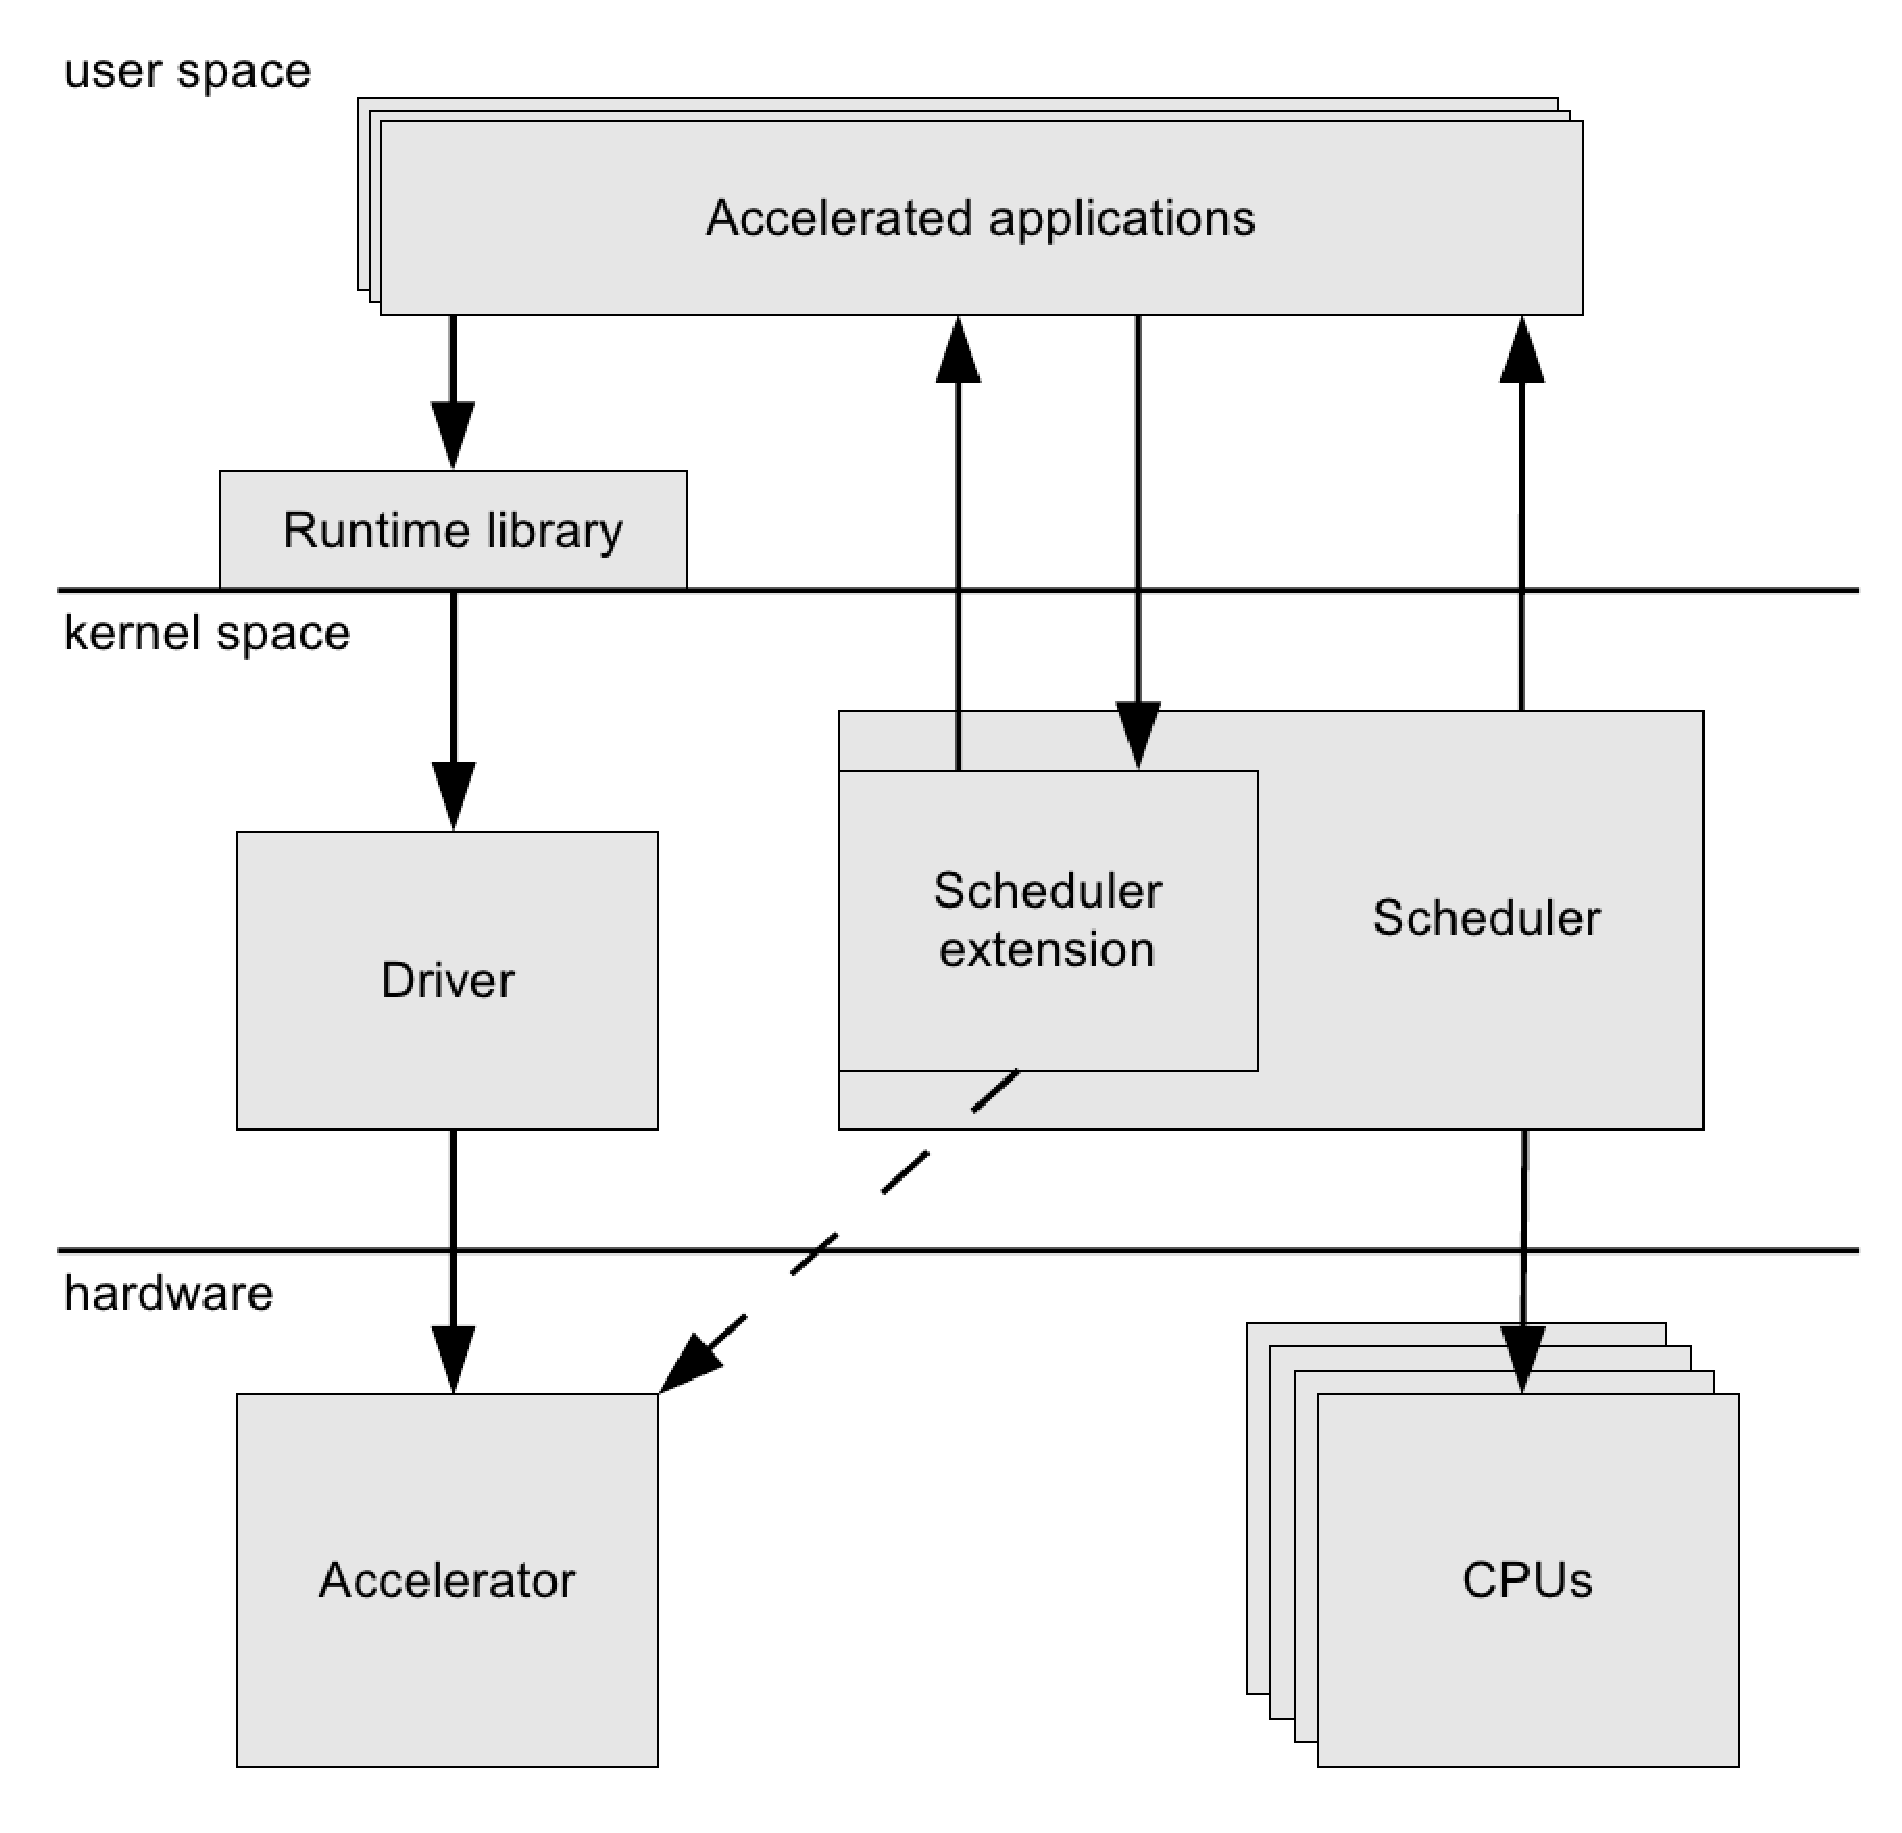
\includegraphics[width=13cm]{eps/schema.eps}
        \caption{Schema of the architecture implemented}
    \end{figure}
    \begin{figure}[H]
        \centering
        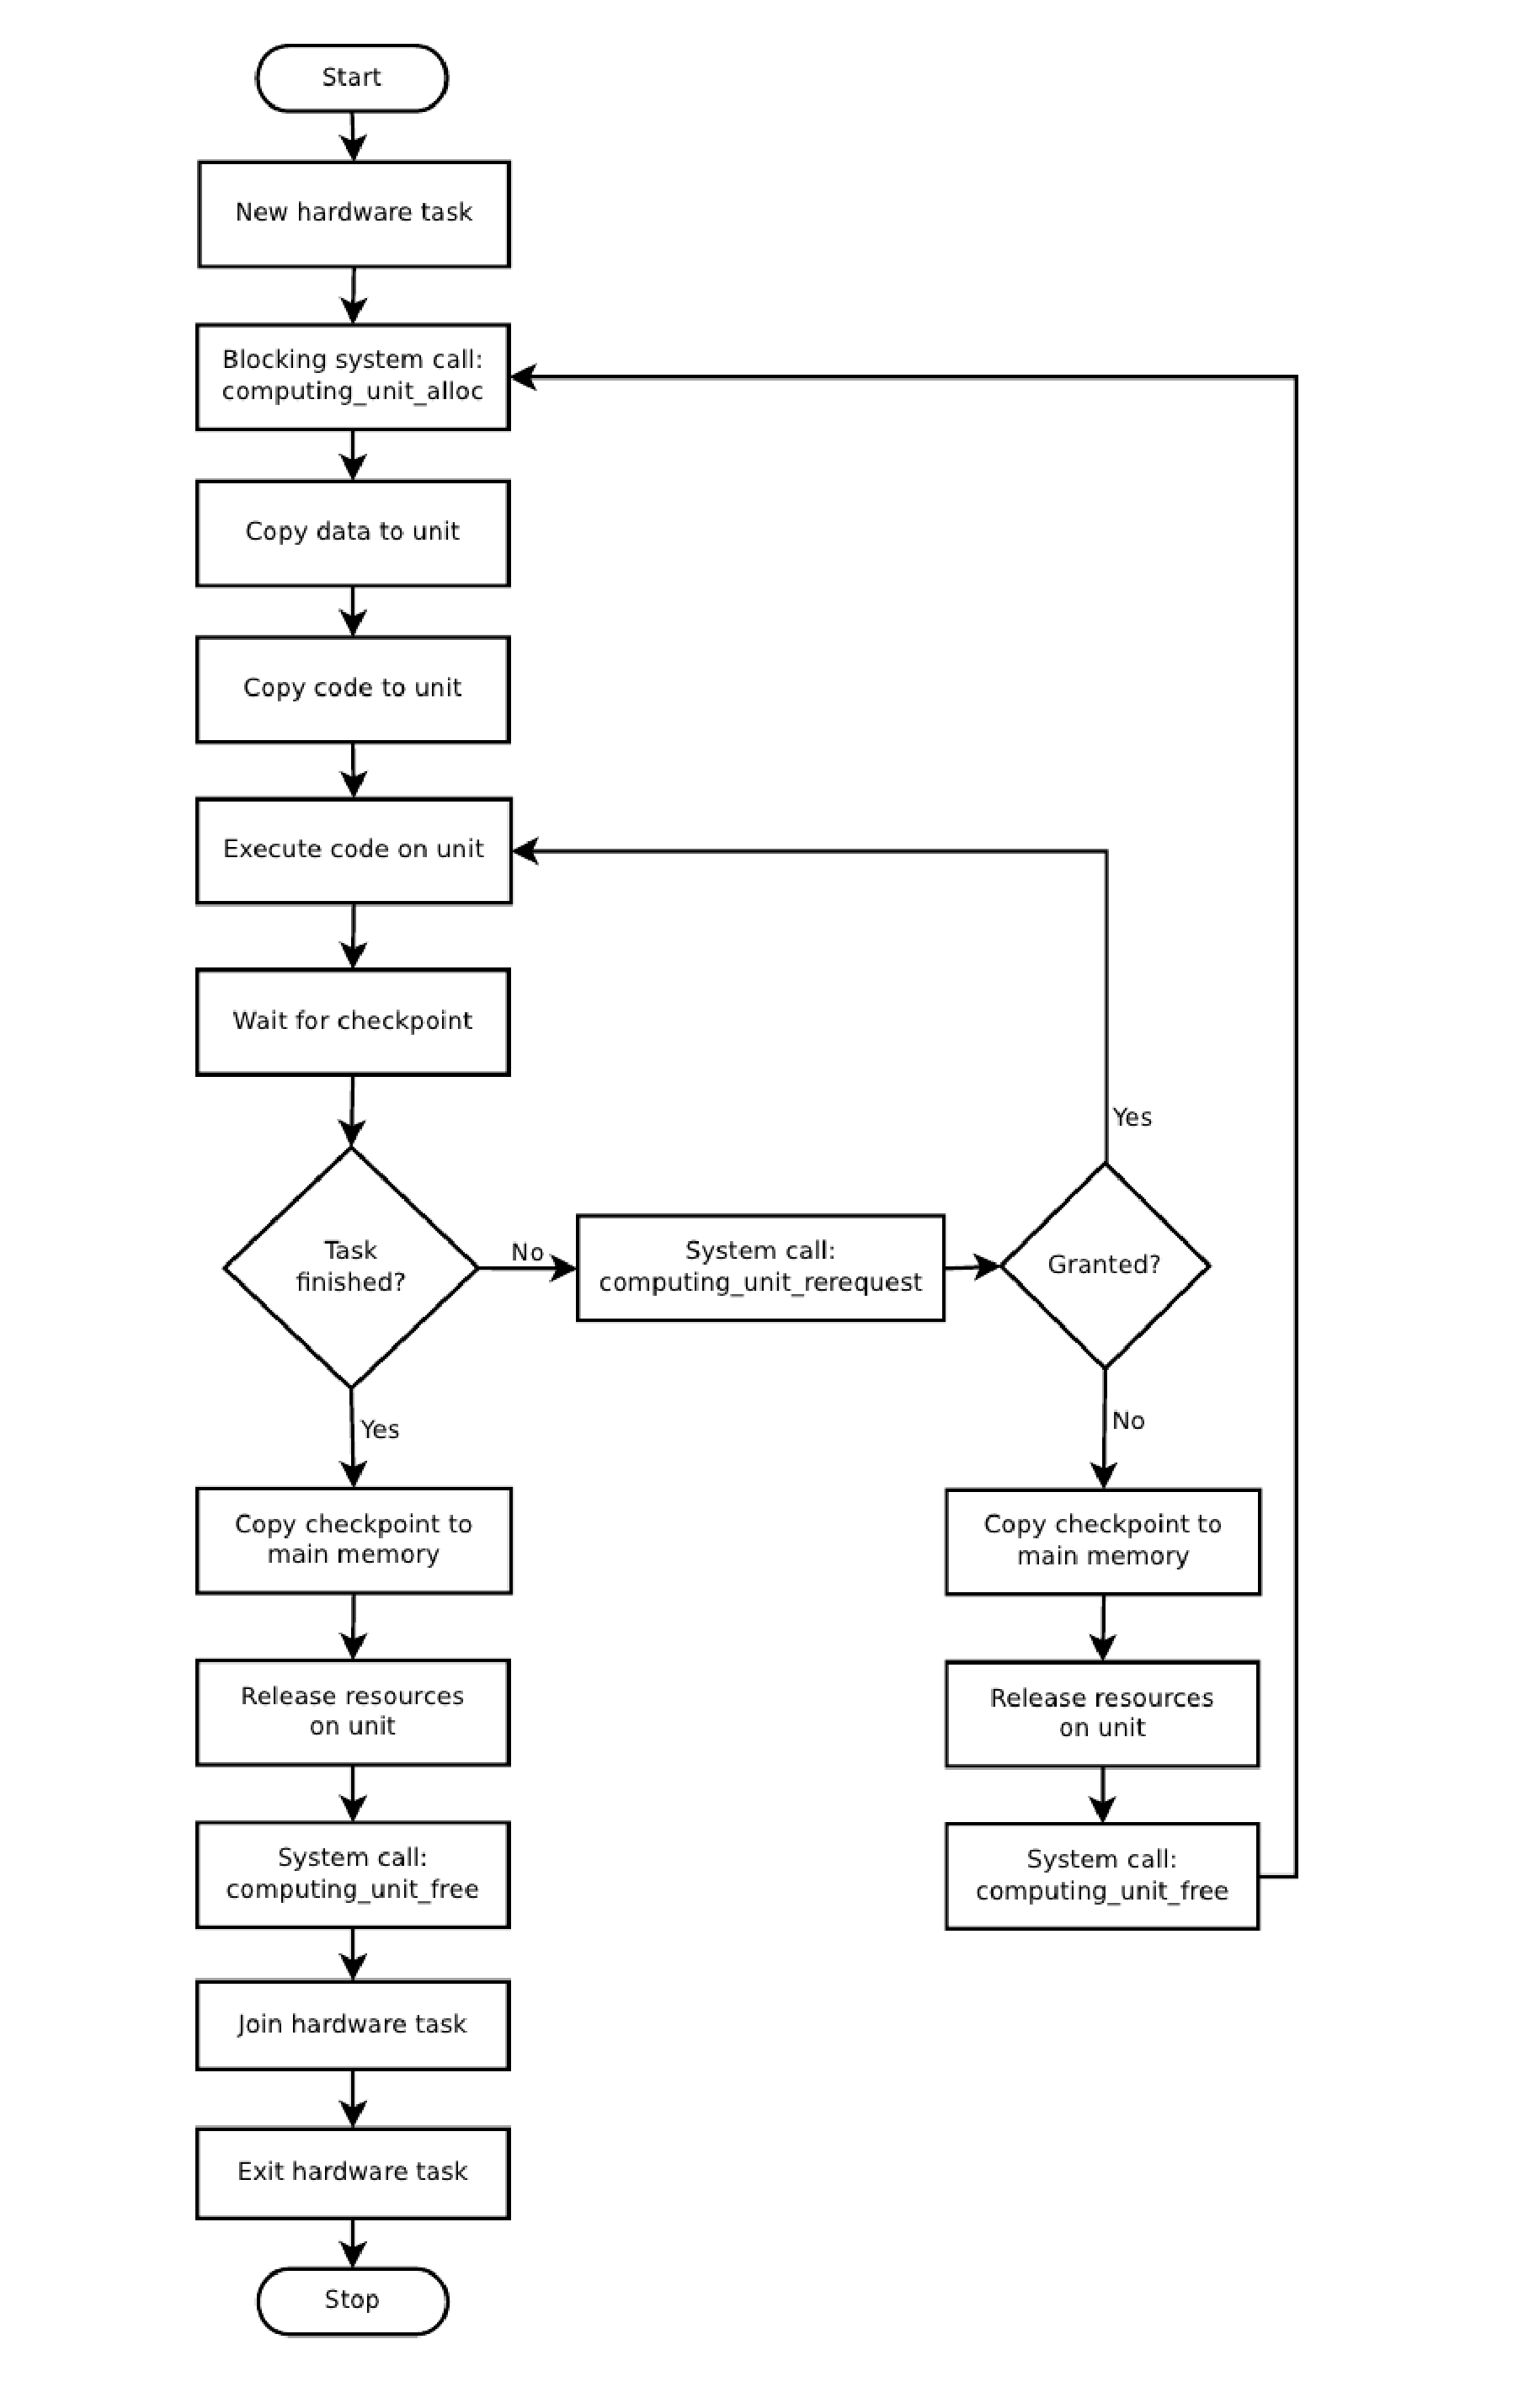
\includegraphics[width=10cm]{eps/flowchar.eps}
        \caption{flowchart of the execution for each process}
    \end{figure}
\begin{multicols}{2}
\vspace{50ex}
\section{Installation Guide}

In this section we will see which steps are needed to setup our linux box to support accelerators.
I will describe where take the files useful to the installation and which components have to be setuped.


\subsection{OS installation and drivers installation}
    Before everything, we have to install the OS. During my project I decided to test it on Gentoo linux 32 bit.
    I had problems with it because NVIDIA doesn't release official drivers for that specific distro and the drivers
    provided by the gentoo developers did not work properely to this kind of application. So I decided to move
    everything on the Operating System used by the authors.
    This hybrid scheduler has been built on a Ubuntu 10.04.4 LTS.
    You can download the ISO image from the following link\\
    \href{https://mega.co.nz/#!IodSWLZS!FHynfh_DNqm0Kb1rWb9ckX_uT68BPhaFthWQh34EuWk}{Ubuntu ISO Image}\\
    Either burn it on a cd-rom (using eg. k3b, brazero) or create a bootable pendrive (look at this guide \href{https://help.ubuntu.com/community/Installation/FromUSBStick}{FromUSBStick})\\
    Install the Ubuntu distro on a either a laptop or a PC where is plugged in an accelerators (in our specific case an NVIDIA graphics card)
    To do  so look at the \href{https://help.ubuntu.com/10.04/installation-guide/i386/}{Ubuntu 10.04 Installation Guide}\\
    Ubuntu as default installs non-proprietary drivers (nouveou) that don't allow to program the graphic card. We have to remove them and install the proprietary driver provided from nvidia.
\end{multicols}
\begin{figure}[H]
\centering{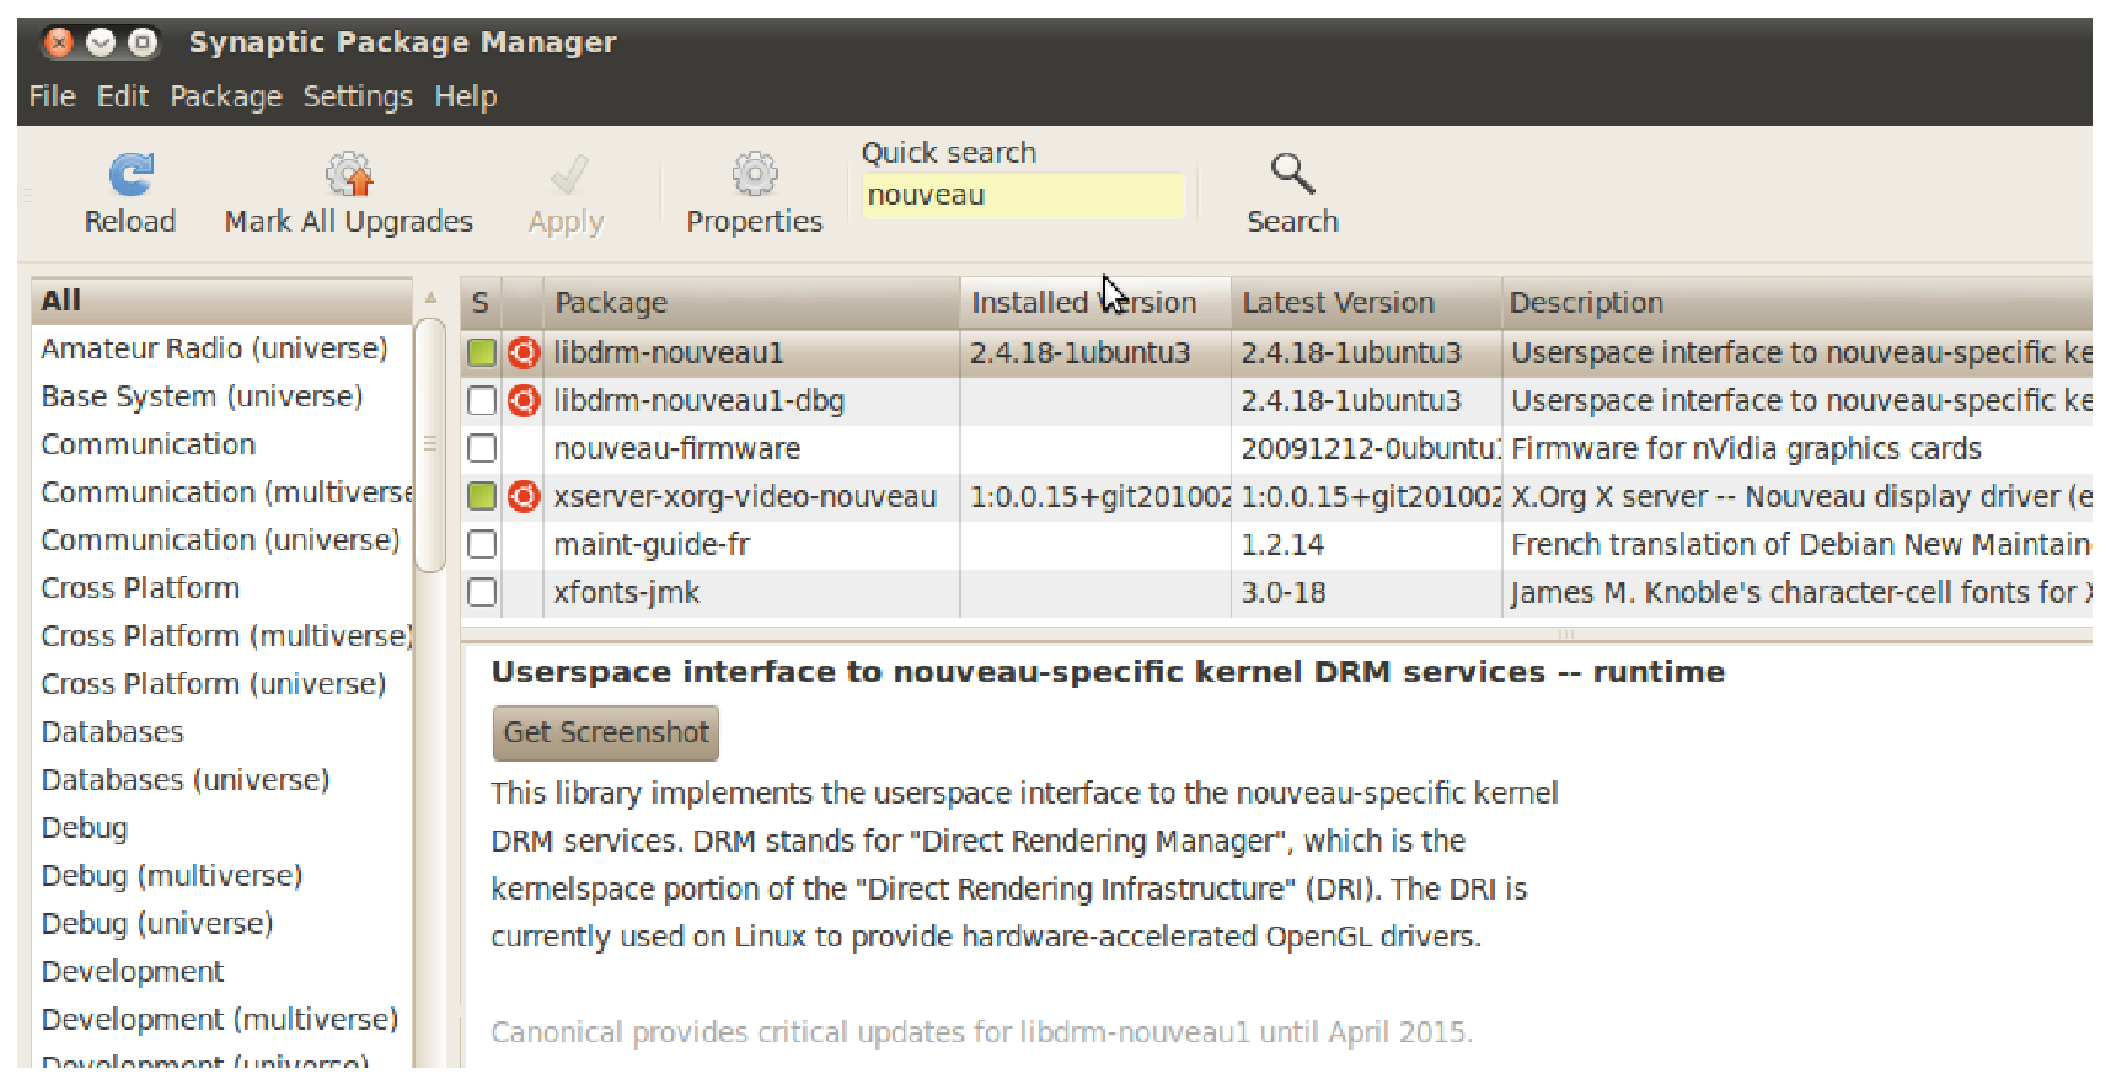
\includegraphics[width=13cm]{eps/nouveau_small.eps}}
\caption{Disinstalling nouveou driver (nouveau-firmware package) using the Synaptic Packege Manager }
\end{figure}
\begin{multicols}{2}
    This scheduler has been developed in 2010 when the driver version was 3.1. I tried to use it with the most recent 5.0 but given a possible change to the APIs it returns a runtime error.
    The driver that I used are downloadable from \href{https://mega.co.nz/#!g49wnBaR!eVaf8DeGmDyPUV8VoJMtHRAHXDE4_-EWxwrmL6LCHWY}{NVIDIA dev-driver 3.1}\\
    To install it run in a terminal as root the commands (NB the X server has to be shutted down)
  \lstset{language=bash}
  \lstset{
      basicstyle=\ttfamily\footnotesize,
          breaklines=true,
          tabsize=2,
          showspaces=false,
          showstringspaces=false,
          framexleftmargin=5pt,
          framexrightmargin=5pt,
          framexbottommargin=5pt,
          framextopmargin=5pt,
  }
   
\begin{lstlisting}
#chmod u+rx devdriver_3.1_linux*.run
#./devdriver_3.1_linux_32_256.40.run
\end{lstlisting}
    The second step to have our cuda framework working is to install the \href{https://mega.co.nz/#!d1FD0TiS!PusMUXIuLJzxiM_hh4ABi1ltWvAIARZutZR3wIR4TEU}{NVIDIA SDK}\\
    The commands to install it are
\begin{lstlisting}
#chmod u+rx gpucomputingsdk*.run
#./gpucomputingsdk_3.1_linux.run
\end{lstlisting}
    Are useful but not necessarily the toolkits provided by nvidia downloadable from \href{https://mega.co.nz/#!88kFCCJL!FmqUdQHY0VE00V5aQOcTQRuaufw9bZ6AS7ZyfQGXiSc} {Toolkits}\\
    As before to install the toolkits run the commands
\begin{lstlisting}
#chmod u+rx cudatoolkit_3.1*.run
\end{lstlisting}
    We can use the following commands to check if the drivers and the tools are correctly installed
    \begin{itemize}
        \item{{\bf nvcc} is the most important tool. It's the NVIDIA compiler for cuda}
            \begin{figure}[H]
                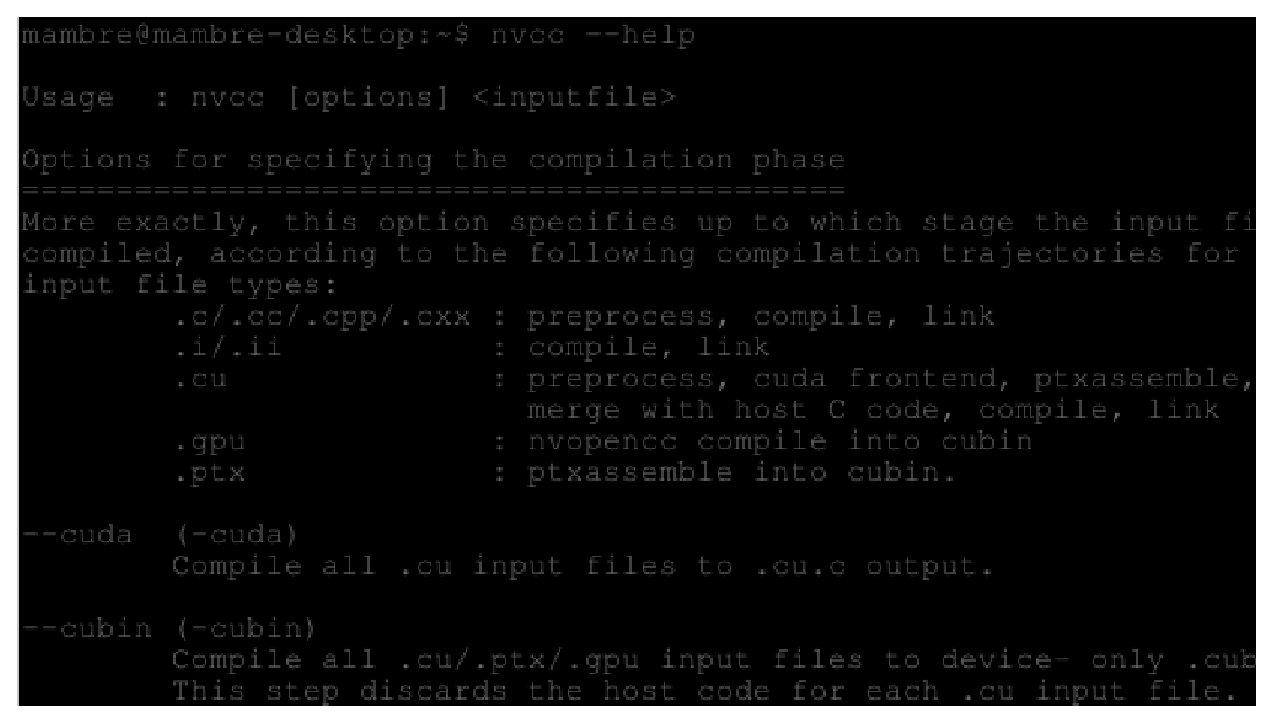
\includegraphics[width=8cm]{eps/nvcc.eps}
            \end{figure}
        \item{{\bf nvidia-smi} allow us to see which graphic units are installed on our machine}
            \begin{figure}[H]
                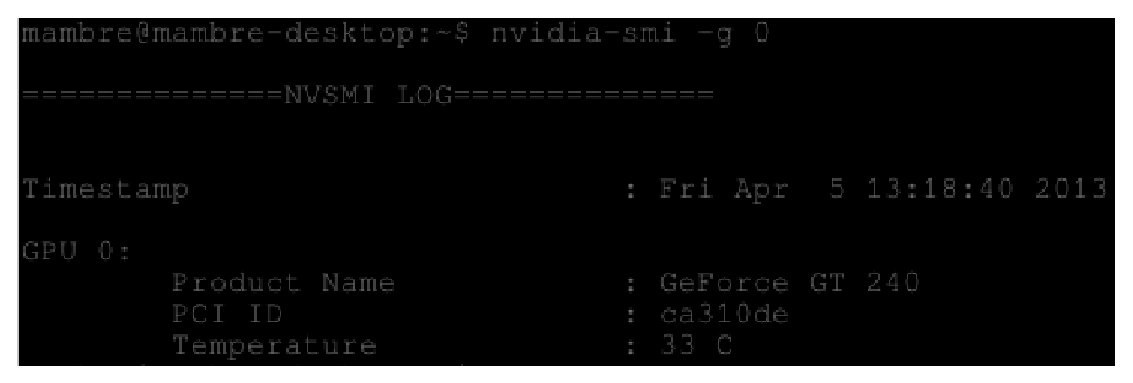
\includegraphics[width=7cm]{eps/nvidia-smi.eps}
            \end{figure}
        \item{{\bf lsmod} program let us know if the kernel module 'nvidia' is loaded and used by the linux kernel}
            \begin{figure}[H]
                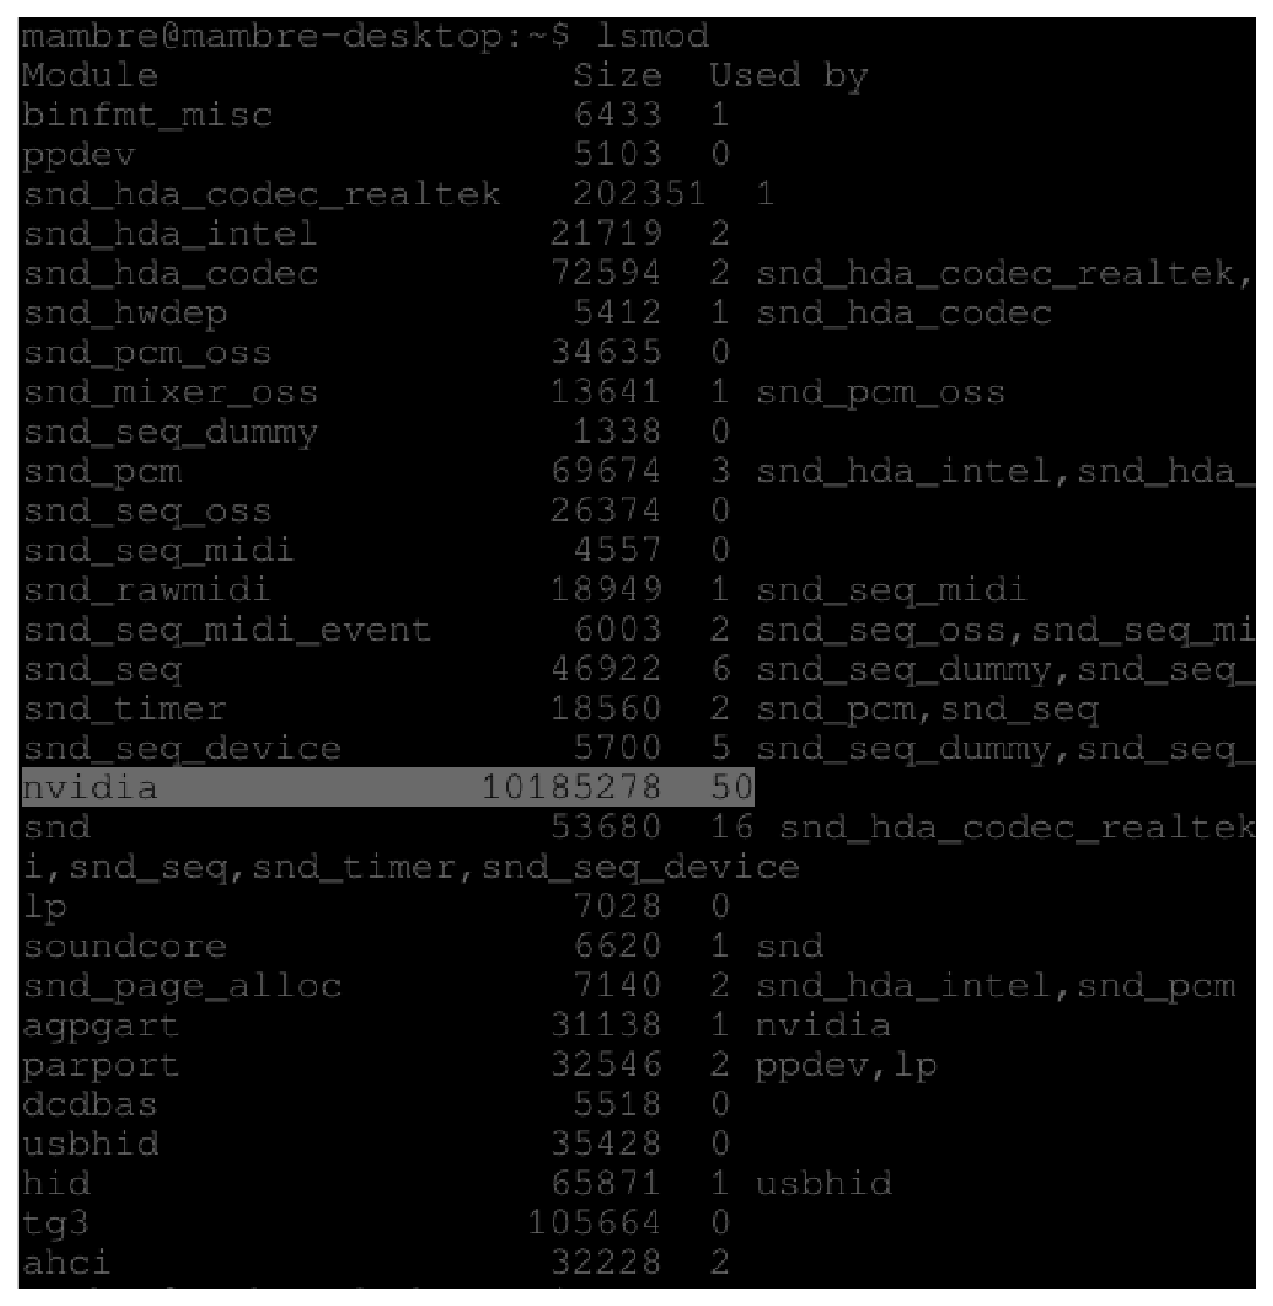
\includegraphics[width=7cm]{eps/lsmod.eps}
            \end{figure}
    \end{itemize}

\subsection{Kernel download and patching}
    Now that we have the OS properely installed and configured we have to download the \href{www.kernel.org}{kernel}\\
    Either we download the tar.gz of  the right version (2.6.32.57, skip the first list of commands look at only the patch) or we clone the git repository running the following commands (The hardest way):\\
    \begin{lstlisting}
#cd /usr/src/
#git clone git://git.kernel.org/pub/scm/linux/kernel/git/stable/linux-stable.git linux-stable
#git checkout v2.6.32.57
#rm /usr/src/linux && ln -s /usr/src/linux-stable /usr/src/linux
    \end{lstlisting}
    With the last command above we move our history at the tag of the right version for the patch provided 
    by the author.
    Now we have to download in the /usr/src/linux-stable/ folder the patch. Use \href{https://mega.co.nz/#!R09hlSrY!TjYiR2m4xV6hadBFEuXAQ2r1-TBUB4LIkAU7-0sgn58}{this link} to retrive the patch 
    The command below apply the patch to the kernel:
\begin{lstlisting}
#patch -p1 < kss_2.6.32.57.patch
\end{lstlisting}
    We have done with the hardest way to do that. I have already done all those things and are stored in my github repo
    so easily you can choose to clone my repo with the patch already applied:
\begin{lstlisting}
#cd /usr/src/
#git clone https://github.com/m4mbr3/RTOS_kernel.git linux-patched
#rm /usr/src/linux && ln -s /usr/src/linux-patched /usr/src/linux
\end{lstlisting}

\subsection{Kernel setting, compilation and installation}
    In this phase we have the kernel correctly installed but it is not configured. I have copied the
    .config file precreated by ubuntu. It is general with all the most common modules. If you want
    to create your own kernel config file run: 
\begin{lstlisting}
#make menuconfig 
\end{lstlisting}
    Select all the components of your machine. Save it. Now you are ready to compile the kernel.
    Run:
\begin{lstlisting}
#make -jX
\end{lstlisting}
    The X has to be changed with the number of your cores + 1. It makes the compilation faster. If you prefer to 
    have a one core compilation just remove it. In this case only one thread will be processed at a time.
    Before 'make' starts to compile it asks you to set some variables releated to the extension.
    It asks to set the following parameters:
\begin{lstlisting}
1) CU_HW_QUEUE_LIMIT
2) CU_HW_LOAD_BALANCER_FILLS_QUEUE
3) CU_HW_KEEP_QUEUE_FULL
\end{lstlisting}
    They are also tunable in
\begin{lstlisting}
'include/linux/sched_hwaccel.h'
\end{lstlisting}
    The firt one sets the limit, the second one controls if the load balancer should refill the queue once 
    it runs and the third one controls if the load balancer is invoked when the accelerator is idle or when 
    the queue is not full. These parameters are linked to migration modes.
    Listed below the different cases:
    \begin{itemize}
        \item{ {\bf Migration without queue limit:\\}
\begin{lstlisting}
#define CU_HW_QUEUE_LIMIT 99999
//#define CU_HW_LOAD_BALANCER_FILLS_QUEUE
//#define CU_HW_KEEP_QUEUE_FULL
\end{lstlisting}
        }
        \item{ {\bf Migration without queue limit 5 and fixed set of tasks\\}
\begin{lstlisting}
#define CU_HW_QUEUE_LIMIT 5
#define CU_HW_LOAD_BALANCER_FILLS_QUEUE
#define CU_HW_KEEP_QUEUE_FULL
\end{lstlisting}
        
        }
        \item{{\bf Migration without queue limit and variable set of tasks\\}
\begin{lstlisting}
#define CU_HW_QUEUE_LIMIT 5
#define CU_HW_LOAD_BALANCER_FILLS_QUEUE
#define CU_HW_KEEP_QUEUE_FULL
/* Also for this mode is needed  a modification in the file sched_hwaccel.c from */ 
if (is_cpu_cui(cui)||
    cui->cfs_rq.nr_running < CU_HW_QUEUE_LIMIT - 1)
/* To */

if (is_cpu_cui(cui) ||
    cui->cfs_rq.nr_running < CU_HW_QUEUE_LIMIT)
\end{lstlisting}
        }
    \end{itemize}
    There is also another tunable parameters inside the 'kernel/sched_hwaccel.c' file.
    You will find the basic granularity setting per type:
\begin{lstlisting}
static u64 type_granularities_sec[CU_NUMOF_TYPES]
\end{lstlisting}
    Alternatively you can
\begin{lstlisting}
#define APPLICATION_CONTROLLED_GRANULARITY
\end{lstlisting}
    in the previosly discussed header file and thereby extend the signature of the
    allocation system call.

    After the end of the compilation we have to install the kernel and set the grub configuration.
    It is feasible running the commands:
\begin{lstlisting}
sudo make modules_install
sudo make install
sudo update-initramfs -c -k 2.6.32.57
sudo update-grub
\end{lstlisting}
    To check if everything is gone ok reboot the system and select the new voice in the list.
    If you get either a kernel panic or something that doesn't work try a new kernel configuration
    to include the missing parts.
    Instead, if everything seems to go normal go ahead in the configuration.



%codice
\begin{verbatimtab}
\end{verbatimtab}
%how add TODO 
\todo[inline]{Sezione con implementazione e programmi di test}
\todo[inline]{Sezione con guida all'installazione}



%-----------------------------------------------------------------------------

% We suggest the use of JabRef for editing your bibliography file (Report.bib)
\bibliographystyle{splncs}
\bibliography{Report}

\end{multicols}
\end{document}
